\section{Quantum digital signatures}
%This section will basically be my "literature review" section.
%I will focus on the main thread of QDS developments initially, but I can supplement it by including some of the asian papers later.

%Note: after I have this section I can compare it to the Amiri2015 review paper and to Collins2018 progress report (and to Callum's thesis)


\subsection*{Quantum one-way function}
%Talk about Gottesman and Chuang.
Gottesman and Chuang \cite{Gottesman2001} generalized Lamport's scheme \MT{cite} in $2001$ to build the first Quantum Digital Signatures protocol. The key contribution of their scheme is to replace the one-way function in \MT{cite} with a so-called \emph{quantum one-way function}, thereby securing the signatures protocol against a quantum adversary.

\MT{TODO: chat more about quantum one-way function. Include the "figure" that I currently have in my historical introduction}

A direct analogue of public-key cryptography, their protocol relies on the difficult task, described in Fig.~\MT{X}, of accurately distinguishing between non-orthogonal quantum states. Their security relies on the fact that performing measurement on a state of $n$~qubits can yield at most $n$~bits of information, and so the protocol in Ref.~\cite{Gottesman2001} is designed such that this is insufficient to distinguish between states.

The key tool in the protocol is a quantum $SWAP$ test, Fig.~\MT{X}, which probabilistically determines whether two states are identical. To perform this test, players prepare $\ket{f_x}, \ket{f_{x^\prime}}$ and an additional ancilla $\left(\ket{0} + \ket{1}\right)/\sqrt{2}$. Players perform a Fredkin gate \MT{cite} using the ancilla as a control, and then perform a Hadamard \MT{cite} on the ancilla. In other words, the $SWAP$ test performs the mapping
\begin{equation}
\ket{f_x}\ket{f_{x^\prime}}\frac{\left(\ket{0} + \ket{1}\right)}{\sqrt{2}} \mapsto \frac{\left(\ket{f_x}\ket{f_{x^\prime}} \pm \ket{f_{x^\prime}}\ket{f_x}\right)\ket{y_{\pm}}}{\sqrt{2}}
\end{equation}
with $y_+=0$ and $y_-=1$. Finally, the ancilla qubit is measured in the $0, 1$ basis, and since $\ket{0}, \ket{1}$ are orthogonal they can be distinguished.  Therefore if $x = x^\prime$ the coefficient of $\ket{1}$ is identically zero, and so the $SWAP$ test always outputs $\ket{0}$. If $x \ne x^\prime$ outputs either $\ket{1}$ or $\ket{0}$. 

The probabilistic nature of this test will cause participants in the protocol to sometimes mistake distinct states for identical ones, but the probability that this occurs may be estimated. Crucially, the protocol may be proven secure if states are chosen such that this probability of honest failure is smaller than the probability to correctly distinguish between large entangled states of non-orthogonal qubits. 

The protocol is a significant attempt to generalise and translate structures from the field of classical cryptography to the quantum realm, and it sets the pattern for all subsequent QDS protocols, and so it is worth examining the protocol in detail. Alice has a $1$~bit message $b$ which she would like to sign, and send to Bob and Charlie. In the Distribution state, for each $b$ Alice creates $M$ classical strings $k_m^i$, length $L$. Each classical string is mapped to a corresponding quantum state $\ket{k_m^i}$ of $n$~qubits which are chosen to be highly non-orthogonal. Two of each of these quantum states are sent to Bob and Charlie. The quantum states, $4M$ in total, are Alice's public keys which may be freely distributed--and they may even be given to a dishonest external party. The corresponding classical strings $k_m^i$ are Alice's private keys.

Bob and Charlie each receive two of the $\ket{k_m^i}$. They each perform a $SWAP$ test between their two copies of the public key, to check whether individual copies are equivalent. Then, they should perform a $SWAP$ test between one of Bob's keys and one of Charlie's keys, to test whether they received identical keys to each other. If all $SWAP$ tests pass then the protocol continues to the next step, otherwise it aborts. Bob and Charlie should now store the quantum public keys which they hold.

Later, in the Messaging stage, Alice sends $\left(m, k_m^i\right)$. For each of the $M$ strings $k_m^i$, Bob creates $\ket{k_m^i}$ and performs a $SWAP$ test with his corresponding stored quantum state. If his test passes most of the time then he accepts the message as genuine and transferable, and passes $\left(m, k_m^i\right)$ to Charlie who performs similar tests. 

Although laying the groundwork for practical QDS protocols, this original proposal cannot be implemented. The most pressing problem is the requirement for long-term quantum memory. State-of-the-art technology can store a quantum state for \MT{X}, and so long-term storage of many copies of quantum states with many qubits will be technologically challenging. Furthermore, the need for every party to be able to create and distribute the states and the multiple required $SWAP$ tests render this protocol impractical for implementation. 

However, as we shall see, the structure of this protocol is very closely aligned to classical signatures protocols. Since the public keys are truly public (all of them can be handed to Eve). Furthermore, every recipient is given identical quantum public keys and so the number of recipients does not need to be fixed before the start of the protocol. These requirements are subtly changed in later--more practical--QDS protocols. \MT{make sure I talk about this later.}

\MT{Perhaps talk about repudiation somewhere in this section?}

%\subsection{Andersson2006 (+ implementation)}
\subsection*{QDS implementation}
%Talk about Andersson2006 and Clarke2012
A step forward to implementation of QDS occurs in Ref.~\cite{Andersson2006}, in which Andersson \emph{et. al.} replace the tricky to perform $SWAP$ test from Ref.~\cite{Gottesman2001} with a practical state comparison method. The qubits required previously are also replaced by coherent states (qumodes). Combined with the new state comparison scheme, the requirements for QDS have been reduced to just generation and distribution of coherent states and linear optics components (beamsplitters).

\begin{figure}[htp]
\centering
\includegraphics{andersoon2006_state_comparison.png}
\caption{\label{fig:andersson2006_state_comparison}}
\end{figure}

The key step, the comparison of coherent states, is displayed pictorially in Fig.~\ref{fig:andersson2006_state_comparison}. If the photodetector clicks it is a strong indication (a certain indication, in the ideal limit) that $\alpha \ne \beta$. Furthermore this comparison is non-destructive, and simply by placing another beamsplitter in the path of the upper beam, with vacuum input at the fourth port, one recovers $\ket{\alpha}$. Otherwise, for $\alpha \ne \beta$ the output states of the second beamsplitter are identical. This practical state comparison forms the building-block for their QDS protocol. 

\begin{figure}[htp]
\centering
\includegraphics{multiport.png}
\caption{\label{fig:andersson2006_multiport}}
\end{figure}

To allow both parties to perform comparisons, an optical multiport Fig.~\ref{fig:andersson2006_multiport} is used. This allows Bob and Charlie to compare Alice's state declaration with her previously distributed state. It also has the advantage of symmetrizing Bob and Charlie's output states, thus preventing a repudiating Alice. The null ports of the multiport are monitored, since they will click if either Alice is trying to repudiate, or if a malicious party is interacting with the state distribution.

Alice sends coherent states from her alphabet of possible coherent states, both to Bob and to Charlie, and keeps a record of which states she sent. Bob and Charlie feed their states through the shared multiport, thereby ensuring that Alice has sent them identical states (or symmetrizing them if she hasn't), and store their output states in quantum memory. Later, Alice sends the classical message, plus classical information describing which states she had previously sent. Bob and Charlie create the corresponding coherent states, and compare them via the method in Fig.~\ref{fig:andersson2006_state_comparison} with the states retrieved from quantum memory. If no clicks are recorded at the null ports, it is an indication that the message is genuine and the protocol passes.

This protocol was implemented by Clarke \emph{et. al.} in Ref.~\cite{Clarke2012}, where an alphabet with $8$ phase-encoded coherent states was used, and signature lengths $L \sim $\MT{X} were obtained. \MT{I don't think they actually quote one, but I can estimate it from their $g$ value.} To get around the requirement for quantum memory, in Ref.~\cite{Clarke2012} the Messing and Distribution stages occur at the same time so the coherent state corresponding to the chosen private key may be interfered with the distributed quantum signatures. This prevents their scheme from being used in a realistic setting where the Distribution and Messaging stages can typically occur with a delay of days, weeks or even years.




%\subsection{Dunjko2014 (+ implementation}
\subsection*{Removing quantum memory}
The requirement that recipients possess long-term and efficient quantum memory, needed for the above protocols, makes it impractical for realization. The removal of this requirement by Dunjko \emph{et. al.} \cite{Dunjko2014} was one of the major milestones towards a practical QDS which can be implemented. 

The key insight of Ref.~\cite{Dunjko2014} was to effectively replace the quantum public key by a classical one, albeit one which relies on the distribution and measurement of non-orthogonal quantum states. This physical requirement is a practical one, relying on simply linear optics (beamsplitters) and photodetectors capable of distinguishing just between zero and nonzero photon numbers, such as avalanche photodiodes (APDs). The storage of classical public keys is clearly no restriction. 

The main difference then between Refs.~\cite{Dunjko2014} and \cite{Gottesman2001}, is that in Dunjko \emph{et. al.}, recipients Bob and Charlie perform photon-number measurement as they receive the quantum states. Remarkably, despite this fundamental change to the nature of the protocol's one-way function, secure QDS is possible. \MT{do I need to revise this sentence? Is it accurate and fair?}

\MT{Include a figure (minipage thing) comparing the one-way functions used by Gottesman2001 and by Dunjko2014.}

In the Distribution stage of the protocol, Alice generates classical strings $\left\{k_j^m\right\}_{j=0}^L$, length $L$, corresponding to each future one-bit message $m$. The $k_j^m$ are chosen uniformly at random from the BPSK alphabet of coherent state phases $\left\{- \alpha, \alpha\right\}$. Alice then forms sequences of coherent states $\rho = \otimes_{j=0}^L \ket{k_j^m}$ which she then distributes to Bob and to Charlie. 



Bob and Charlie pass their received coherent states through the shared optical multiport, Fig.~\ref{fig:dunjko2014_multiport}, which serves to symmetrize their individual quantum states. That is, after the multiport Bob and Charlie's reduced density matrices are identical, which guards against Alice's repudiation attack. Each recipient has two outputs of the multiport. One output, the so-called "null-port" should be monitored for clicks of the photodiode which imply that $\alpha \ne \beta$ (Bob and Charlie have different coherent states, Fig.~\ref{fig:dunjko2014_multiport}) which may imply the presence of an attack. Bob and Charlie should also perform unambiguous state discrimination (USD) on the outputs of their signal ports, which will accurately distinguish between non-orthogonal states $\ket{\alpha}, \ket{-\alpha}$ at the expense that it will sometimes fail to give an answer. 

During Messaging, Alice will declare $\left(m, k_j^m\right)$ which recipients will compare to their USD outcomes. Provided that there are enough matches between Alice's phase declarations $k_j^m$ and Bob/Charlie's USD outcomes, message $m$ is accepted and the protocol has succeeded.

This first protocol avoiding the requirement for quantum memory shows that QDS may be both practical and secure. Furthermore the limited physical requirements--tensor-products of coherent states, beamsplitters and non-photon-number-resolving detectors--are feasible to work with, unlike the large number of superposition qubits required for Ref.~\cite{Gottesman2001}. \MT{Now talk about the implementation paper}. 

An implementation of a variation of Dunjko's scheme is described in Ref.~\cite{Collins2014}. Collins \emph{et. al.} modify Dunjko's scheme in two key ways. Firstly, a QPSK alphabet Eq.~\MT{X} is used, rather than BPSK. This is in order to make the second modification: instead of using unambiguous state discrimination (USD) measurement, they perform unambiguous state \emph{elimination} (USE) measurement. If the measurement succeeds, rather than being able to say definitively which state was received, a recipient can say with certainty which state was \emph{not} received. This measurement scheme is described further in Fig.~\ref{fig:USE}. The key advantage of the USE measurement scheme is that the probability that the measurement fails is significantly smaller than for USD, and so the resulting QDS scheme gains a boost in efficiency. Indeed, if USE eliminates $N-1$ of $N$ possible states then one knows with certainty which state was sent, USD may be viewed as a special case of the more general USE measurement. The shift from state discrimination to state elimination allows for much greater efficiency in QDS schemes. \MT{Make sure to talk about it later in the context of our QDS - make a graph showing $g$ (or $L$?) under discrimination vs elimination.}

\begin{figure}[htp]
\centering
\includegraphics{USE.png}
\caption{\label{fig:USE}}
\end{figure}

Collins \emph{et. al.} estimate a signature length $L = 5.1 \times 10^{13}$ in order to sign a message. Notice the subtle shift between Refs.~\cite{Gottesman2001} and \cite{Andersson2006, Clarke2012, Dunjko2014, Collins2014}. While previously the number of recipients did not need to be determined until the Messaging stage, here it must be determined before Distribution. After the coherent states have passed through the multiport the number of recipients cannot be changed. 
\MT{I should note later that removing the multiport removes this restriction.} Because of the physical requirements for the optical multiport, it will also be challenging (though possible) to generalize to more recipients, though note that for more than two recipients in Ref.~\cite{Dunjko2014} one may not use $USD$ measurement. \MT{why?}. Realistic implementation of the multiport also introduces noise and losses due to misalignment and instability, further reducing the efficiency of the protocol, and requires Bob and Charlie to be physically connected. In Ref.~\cite{Clarke2012, Collins2014}, for example Bob and Charlie are separated by $5$~m of optical fibre. 

The most difficult assumption which Refs.~\cite{Clarke2012, Dunjko2014, Collins2014} make, however, is that there should be no eavesdroppers on the quantum channels. This is a strong and impractical assumption, and one which subsequent papers endeavour to remove.

\MT{TODO: mention somewhere how Dunjko2014 differs from Andersson2006}

\subsection*{Removing multiport}
%\subsection{Wallden2015 (+ implementation)}

The fact that the QDS schemes discussed above require dedicated hardware at the receivers--the optical multiport--makes implementation in real-world situations difficult. The multiport introduces losses and noise, and requires tricky synchronisation between Bob and Charlie in order to correctly interfere the states. The experiment in Ref.~\cite{Collins2014} therefore has Bob and Charlie only separated by $5$~m optical fibre. 

To combat this, Wallden \emph{et. al.} \cite{Wallden2015} propose two QDS schemes specifically designed to run over the same hardware platform as QKD. In particular, they get rid of the multiport which was previously use to symmetrize Bob and Charlie's reduced output states. Their key insight is that rather than symmetrizing their states, it is sufficient to symmetrize their measurement outcomes. Therefore, a step is added to the distribution stage in which Bob and Charlie randomly swap half of their measurement outcomes over a secure classical channel. If Alice can gain no information about which outcomes were swapped then she cannot repudiate. 

This protocol was implemented by Donaldson \emph{et. al.} in Ref.~\cite{Donaldson2016} in which a message is securely signed over distances $500$~m, $1000$~m, and $2000$~m, with no requirement on the physical separation between Bob and Charlie. The secure classical link may be realised via QKD, and so Refs.~\cite{Wallden2015, Donaldson2016} begin to explore the close connections between these two different quantum communication protocols. We explore this further in Chapter.~\MT{X}. Donaldson \emph{et. al.} achieve signature length $L = 1.93 \times 10^9$ using QPSK coherent states and USE measurement. This is a vast improvement over the $L = 5 \times 10^{13}$ required in Ref.~\cite{Collins2014} and means that secure quantum signatures may actually be both useful and practical. 

\subsection*{Allowing Eve}
%\subsection{Amiri2016 (+ implementation)}
All signature schemes considered so far have made the assumption that the quantum distribution channels are secure, that is, they may not be attacked or monitored by an eavesdropper, Eve. This is clearly an unrealistic and unphysical assumption, but was a sensible one while the pressing impracticalities of early QDS schemes (quantum memory, multiport, tricky state comparison tests) were overcome. The emphasis in earlier papers was on dishonesty internal to the protocol, i.e. which attacks can Bob or Charlie mount when they already hold perfect copies of the quantum public keys. However, in a realistic scenario it is clear that an eavesdropper \emph{could} attack the quantum channels as states are being distributed, and so it is important to consider whether this has any effect on QDS security.

Amiri \emph{et. al.} provide a QDS scheme which allows for an Eve to eavesdrop on the quantum channels. In the worst-case scenario it is assumed that Eve will conspire with a dishonest internal player (Bob or Charlie in the case of a forging attack), and so knowledge which Bob/Charlie hold about their own quantum public key measurements is supplemented by knowledge learned through Eve's attack. For short, we describe Bob or Charlie as performing the eavesdropping attack, so as not to confuse the nomenclature. 

The key modification which Ref.~\cite{Amiri2016} makes is to have Alice use \emph{different} private keys (and so different sequences of quantum coherent states) for each recipient. This means that the dishonest recipient is forced to eavesdrop on the honest recipient's quantum channel if he is to gain any information. This is in contrast to earlier protocols in which the dishonest recipient held a perfect copy of the quantum public key, which was identical to that of the honest recipient. 



The protocol relies on sending weak attenuated coherent states, identically to decoy-state BB$84$ \MT{cite}, with three different intensities. The coherent states are randomly polarized in one of two orthogonal polarization bases, and single-photon detection in one (randomly chosen) polarization basis is performed at the receiver. The three different intensities are required in order to circumvent a photon-number splitting attack \MT{cite}. Players gain classical binary strings, which are later compared during the Messaging stage. The protocol is secure provided that Bob's (Charlie's) string is closer\footnote{in Hamming distance} to Alice's string than any possible string which a dishonest eavesdropper can hold. 

Because the security of discrete-variable QKD is so advanced, the QDS protocol proposed in Ref.~\cite{Amiri2016} is secured against coherent eavesdropping attacks\footnote{We will discuss the hierarchy of eavesdropping attacks in Sec.~\MT{X}} via an estimation of the smooth-min entropy \MT{cite}, which is the commonly bounded quantity for analysis of quantum cryptographic protocols. Amiri \emph{et. al.} note specifically that the quantum stages of their protocol are identical to the equivalent QKD protocols, with difference only in the classical postprocessing of measurement results. This becomes a common factor of many QDS protocols as they move towards realistic and practical implementation, even in commercial systems and installed fibers, and is a thread which we shall pick up again in Ch.~\MT{X}.

Because the dishonest player is forced to eavesdrop, he in fact receives a worst copy of the honest player's public key than in the above protocols, and so somewhat counter-intuitively Ref.~\cite{Amiri2016} requires only an estimated $L = 6\times 10^8$ over $50$~km fiber. Remarkably, this is \emph{shorter} than previous protocols, despite relaxing a security assumption.

An experimental implementation of a protocol which is similar to Ref.~\cite{Amiri2016} is descried in Ref.~\cite{Yin2017c}, based on the protocol Ref.~\cite{Yin2016a}. This protocol relies on distribution of decoy-state BB$84$ (attenuated coherent states of several different polarizations, as with Ref.~\cite{Amiri2016}). The crucial differences between Refs.~\cite{Amiri2016} and \cite{Yin2017c, Yin2016a} are that \cite{Yin2017c, Yin2016a} use a larger set of (non-orthogonal) polarization bases, and that \cite{Yin2017c, Yin2016a} requires no swapping between Bob/Charlie, and requires Alice to send the same sequences to Bob/Charlie. Yin \emph{et. al.} sign a $32$~bit message over a distance of $102$~km, making their experiment the longest implemented message to-date.



Finally, we note the recent work by An \emph{et. al.} \cite{An2019} which boasts an experiment with GHz clock rate based on Ref.~\cite{Amiri2016}, allowing for coherent forging attacks by Eve and requiring single-photon detectors at the receiver.


\subsection*{Side-channel attacks}
%\subsection{Puthoor2016 (+ implementation)}
%\MT{Though first talk about side-channel attacks}
It should be noted that "security" of a protocol is a theoretical statement, and not a physical one. A protocol is secure with respect to a model of how it operates in the real world, and whether a so-called unconditionally secure protocol can be broken in practice depends on how realistic or practical its underling modelling assumptions are. For example, although in many QKD protocols Eve is allowed to attack the quantum channels and eavesdrop on all communication, she is prevented from attacking the physical devices which are used to implement the protocol. 

For example, the QDS scheme presented in Ref.~\cite{Amiri2016} relies on distribution and detection of quasi-single photons \MT{make sure I have discussed this earlier} in different polarization bases. Physically, Alice must prepare her states before they are sent. A realistic Eve could attack Alice's device in order to gain information about the polarization of the prepared state and so she might gain enough information to forge without detection, even though the protocol is unconditionally secure against conventional types of eavesdropping attack.

An example of such a side-channel attack \MT{define what is a side-channel attack} is the "trojan horse" attack presented in Ref.~\cite{Jain2014}. Here, Eve shines a bright laser pulse into Alice's device and measures the few back-reflected photons which are scattered back. These photons have picked up the same polarization as Alice imparted to her prepared state, and so Eve is able to infer the chosen polarization basis choice, which gives her an undetected advantage. Another potential side-channel attack is that information about the intensity-modulation of the weak attenuated coherent states in Ref.~\cite{Amiri2016, Yin2016c} may be leaked.



To guard against side-channel attacks, honest parties have several options. One direction is to close known side-channels by additional protocol steps or additional hardware. Leakage of intensity-modulation information may be removed by using a passive decoy-state scheme, as in Ref.~\cite{Zhang2018}, which uses a parametric down conversion (PDC) source to generate photon pairs. The idler is used to estimate channel parameters, much like decoy intensity modulations were earlier \MT{make sure I talk about this}, and the signal is projected into different non-orthognal polarization states. Although Zhang \emph{et. al.} reach channel distances of $200$~km, they require single-photon detectors cryogenically cooled to $2$~K, and so it is difficult to see how this protocol could be implemented in a real-world scenario.


With the trojan horse attack Alice and Bob could add additional filters to their devices to block out light at Eve's required wavelength. It was shown however that Eve can bypass these filters by breaking Alice's filters, in a way that is undetectable to honest players \MT{cite the laser damage paper}. Closing side-channels in this way may open up the protocols to additional attack methods, which must then be understood, modelled and reacted-to. This places quantum cryptography into the same "cat-and-mouse" development cycles as conventional cryptography. \MT{expand on this, and make sure I have discussed it earlier in the historical overview.}

To break this cycle, and to provide genuinely unconditional security, guaranteed against all conceivable side-channel attacks, there has been a recent push towards device-independent cryptography. The security of device-independent (DI) protocols makes no trust assumptions about the devices used and it may even be assumed that the  devices are held by the malevolent party. DI cryptography is then based entirely on laws of quantum mechanics, specifically on the violation of a bell inequality. \MT{cite some stuff, and expand this paragraph.}

Full DI cryptography, while secure, is difficult to perform and may offer figures of merit which are too pessimistic for the desired application. One may compromise, then, and instead implement measurement device independent (MDI) cryptographic protocols, in which no trust assumptions are placed on the measurement devices (and they can even be owned by Eve), while the state-preparation and sending devices are held by honest parties and are trusted. \MT{cite some papers}

The first MDI QDS scheme is presented by Puthoor \emph{et. al.} in Ref.~\cite{Puthoor2016}, which requires only a characterization of the states which are distributed through the quantum channel, and which places no assumptions on the detectors. The setup of Ref.~\cite{Puthoor2016} is depicted in Fig.~\ref{fig:puthoor2016_setup}. Each player shares a quantum channel with Eve, while message recipients Bob and Charlie share an MDI-QKD link which is used to securely symmetrize their measurement results. This protocol runs similarly to Ref.~\cite{Amiri2016} and differs only in the quantum steps used to distribute correlated classical strings between players. 

\begin{figure}[htp]
\centering
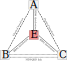
\includegraphics{puthoor2016_setup.png}
\caption{\label{fig:puthoor2016_setup}}
\end{figure}

The correlated strings are shared between Alice and Bob as described in Fig.~\ref{fig:puthoor2016_mdi}, while identical steps are followed to share between Alice and Charlie. Alice and Bob each prepare polarization-encoded Fock states with different intensities, and send them to Eve. If Eve is honest she will perform a Bell measurement \MT{define} on the states which she has received. An honest or dishonest Eve then publicly announces whether the measurement was a success, and the Bell state which she has obtained.

Alice and Bob then communicate to each other their intensity and basis settings (but not the states which they each sent). This allows them to deduce each other's sent state, from Eve's Bell state declaration. Intuitively, since Eve claims to perform a Bell measurement, Alice and Bob \MT{talk about intuitive security of MDI stuff.}

\begin{figure}[htp]
\centering
\includegraphics{puthoor2016_mdi.png}
\caption{\label{fig:puthoor2016_mdi}}
\end{figure}


There have been two main implementations of MDI-QDS. One experiment by Roberts \emph{et. al.} implements either MDI-QDS, MDI-QKD or regular QKD with a switchable setup \cite{Roberts2017}. By handing the untrusted measurement device to Charlie, and allowing Bob and Charlie to additionally share a QKD link, they securely sign a message between Alice and Bob situated $50$~km apart. They also only require two quantum links, between Alice-Charlie and Bob-Charlie (the same as Fig.~\ref{fig:puthoor2016_mid} with Charlie playing the role of Eve), which reduces the resource cost of distributing signatures across a network. Roberts \emph{et. al.} sign a single-bit message in just $74$~ms. 



\subsection*{Installed fibers}
There have been several experiments seeking to move secure QDS from the laboratory setting to a practical network of deployed fibers. The first demonstration of QDS over installed fibers allowed for a single-bit to be signed in approximately one second over $90$~km fiber, relying on a differential phase shift (DPS) quantum state distribution, Fig.~\ref{fig:collins2016_dps}.

In this DPS-QDS protocol, \MT{describe how the protocol runs} 
Key to the long distances reached in this protocol is the move to telecom wavelengths $1550$~nm, allowing the use of very low loss fibers. 

\begin{figure}[htp]
\centering
\includegraphics{collins2016_dps.png}
\caption{\label{fig:collins2016_dps}}
\end{figure}


H.-L. Yin \emph{et. al.} in a second implementation of MDI-QDS \cite{Yin2017} securely sign a message over a deployed fiber network in approx. $40$~hours using the protocol from Ref.~\cite{Puthoor2016}. Yin \emph{et. al.} note that a full parameter optimization was not performed. Regardless, there has been quick and marked progress from early QDS experiments, assuming quantum memories and tricky detection methods which were unique to QDS, to the recent experiments demonstrating unconditionally secure MDI-QDS over installed metropolitan fiber communication systems.

Both of these schemes, although running over deployed fiber networks, require difficult detection methods. Collins \emph{et. al.} \cite{Collings2016} rely on single-photon detectors, while Yin \emph{et. al.} \cite{Yin2017} is required to perform Bell measurements. Both of these require dedicated hardware not normally present in a standard deployed telecommunications network.






%\subsection{Tokyo installed fibers scheme}
%\MT{Perhaps the rest of the DPS-based protocols, or installed-fiber protocols here too?}

\MT{Talk about other QDS implementations}

%\MT{Where shall I talk about An2019?}

\subsection*{Continuous-variables}
\MT{Motivate CV and then talk about Croal2016. Goal of section is to convince the reader that CV QDS is a good direction to go in, and to motivate the rest of the chapter.}

Despite the many recent advances in single-photon detection, and its use above in modern QDS progressing towards practical implementation, the protocols presented above still require a dedicated hardware platform. Deploying such a platform will be difficult and costly, especially if it requires new network infrastructure.

An alternative approach is to build quantum cryptographic protocols specifically designed for integration with the classical telecommunications network. We are therefore motivated to introduce the following comparison between the so-called "discrete-variables" (DV) and "continuous-variables" (CV) approaches to quantum cryptography, Tab.~\MT{X}. \MT{I can have a nice table laying out some of the main differences.} 

The protocols discussed above, relying on single-photon detectors which give a discrete outcome (click or no click), fall within the discrete-variables category. These protocols boast a high level of theoretical development and mature security proofs, owing in part to the small Hilbert spaces in which their systems live. It should be no surprise, therefore, that while many protocols for quantum information processing are designed first for DV systems, they are often implemented first on a CV platform. Quantum teleportation is a good example of this. \MT{cite some stuff.}

CV quantum cryptography, relying on distribution of phase-encoded coherent states and heterodyne detection typically requires complex security proofs. An important issue is the infinite-dimensional Hilbert spaces in which the quantum states live. There are many properties of quantum states which hold for any finite dimension but which break in the infinite dimensional case. \MT{cite some stuff.} Additionally, numerical methods which work efficiently at low dimension \MT{cite some SDP stuff} cannot be implemented in the infinite-dimensional case without simplifying assumptions.

Despite this, the CV platform has preferable implementation. \MT{cite and talk about some developments in CV QKD.} Optical homodyne and heterodyne detection are mature technologies routinely used throughout currently deployed telecommunications networks, and they can run at GHz (or larger) clock-rates. Furthermore, these detection methods are highly efficient \MT{cite} and run at room temperature. One is therefore motivated to pursue CV cryptography by the allure of its technological maturity and compatibility with already deployed architecture. 

The first CV QDS protocol was proposed in Ref.~\cite{Croal2016} by Croal \emph{et. al.} This protocol relied on distribution of QPSK coherent states Eq.~\MT{X}, Fig.~\MT{X} and heterodyne detection of their phase. The structure of the protocol is similar to those discussed previously. Alice first, for each future one-bit message she might send, creates strings of classical information corresponding to a phase from the QPSK alphabet. She then creates sequences of the corresponding phase-modulated coherent states, and sends them through the quantum channel to recipients Bob and Charlie.

Bob and Charlie perform heterodyne measurement and receive a phase measurement outcome. Unlike the schemes discussed earlier implementing an unambiguous state discrimination \MT{cite} or unambiguous state elimination \cite{Donaldson2016}, the measurement used here may be interpreted as an "ambiguous state elimination" (ASE), which is a natural next step in the progression USD $\rightarrow$ USE $\rightarrow$ ASE. The heterodyne measurement outcome is used to eliminate one of the possible QPSK states, similar to Ref.~\cite{Donaldson2016}. But while the USE will always give the correct outcome (i.e. it will never eliminate the state which Alice has sent) at the expense of sometimes failing to give any outcome, in the ideal setting the ASE here will never fail to give an outcome, at the expense of sometimes eliminating the state which Alice did indeed send. So, while in protocols \MT{cite} the ideal minimum number of errors between honest parties is zero, here there will always be a minimum threshold of errors between honest parties--even in the ideal case.

\MT{talk about the experiment}
Croal \emph{et. al.} implement their scheme over a $1.6$~km free-space channel, which makes Ref.~\cite{Croal2016} both the first demonstration of CV QDS and the first demonstration of free-space QDS. Surprisingly, the experiment reaches shorter signature lengths, $L = 7 \times 10^4$ to sign a one-bit message than previous protocols. This is partly due to the ASE measurement scheme, and partly due to the technological maturity of the CV experiment and hardware. Because of the short signature length and the experimental clock-rate, Ref.~\cite{Croal2016} additionally boasts the shortest required time to sign a single-bit message, a fact which is noted in the reviews Refs.~\cite{Collins2016, Collins2018}.

Despite these advances in CV QDS, Ref.~\cite{Croal2016} still makes the assumption that there can be no eavesdropper on the quantum channel. One of the main results of this Thesis is to relax this assumption, as performed in our recent work Ref.~\cite{Thornton2019}. We will discuss this further in Ch.~\MT{X}.

The CV quantum cryptographic platform typically boasts fast sending rates and ready implementation with deployed network architecture, at the expense of being highly sensitive to channel loss and noise. The distances over which CV quantum cryptography is secure are limited, and so the conventional wisdom is that a future quantum cryptography network should use the fast CV protocols over short distances (metropolitan distances within cities would be a perfect application of this), while long-distance quantum communication should be performed using a DV protocol. It is for this reason therefore that the long-distance records for quantum information processing are held by DV protocols \MT{cite some stuff, including the satellite.}



\subsection*{Other directions}
\MT{Talk about "classical" unconditionally secure signatures, and various extensions to the QDS schemes discussed above. I want the above narrative to be about the flow from impractical (Gottesman2016) to practical and good (my scheme, which I am about to present).}


%
%\subsection{"Classical" unconditionally secure signatures}
%\MT{Talk about protocol P2 from Wallden2015, and also Amiri's scheme}
%
%\subsection{Extensions to signature schemes}

Before we move on, it is worth spending a moment to acknowledge some directions of QDS research which are orthogonal to the impractical $\rightarrow$ practical narrative presented above.


\subsubsection*{Unconditionally secure classical digital signatures}
It is important to note that unconditionally secure \emph{classical} digital signatures schemes do exist \MT{cite some stuff.} For example, the protocol P$2$ proposed by Wallden \emph{et. al.} \cite{Wallden2015} offers unconditional security requiring only preshared classical keys. Similarly, the protocol \cite{Amiri2016a} uses \MT{X} to securely sign a message, and protocol \MT{cite the unconditionally secure one based on a trusted third party} can securely authenticate \MT{(and sign?)} a message. All of these are unconditionally secure against even a quantum adversary.

Therefore, one may rightly ask why a future quantum-secure cryptographic network should not use one of these classical protocols. Indeed, there may be applications where one of these protocols is preferable to any quantum protocol. However, it is worth considering the full practical requirements of these protocols. For example, protocols \cite{Wallden2015, Amiri2016a} each require secret preshared keys between all players. These keys could be shared via example \MT{cite computationally secure key sharing protocol}, but in this case the signatures scheme will become only computationally secure. Unconditional security therefore realistically assumes QKD between participants in order to securely share the secret keys before the classical signatures protocol may be run. We may therefore denote these "classical" unconditionally secure schemes as "\emph{indirect} quantum digital signatures", as in practice they will require first the distillation of secret keys (via QKD) and then classical postprocessing. It is not clear \emph{a priori} whether this will be more or less resource intensive than the "direct" QDS schemes above, which perform the signatures task without first distilling secret keys.

Similarly, the unconditionally secure classical digital signatures protocol in Ref.~\MT{cite} relies on a trusted third-party. This is a strong assumption which one may choose to make in some contexts, but it is an open question whether there exist unconditionally secure classical schemes which do not make this trust assumption.

\subsubsection*{Post-quantum cryptography}
What if a user does not require full unconditional security against an infinitely powerful quantum adversary? It may be suitable in some texts to rely on a signatures protocol for which it is merely difficult (not impossible) for a quantum adversary to succeed. Such schemes fall within the remit of post-quantum cryptography, a field whose goal is to design completely classical protocols which should be computationally secure against a quantum adversary. 

Such schemes should be based on a hard problem which is thought to be hard also for a quantum computer\footnote{\MT{Make a statement about how this is not an easy task, since it is not yet known which problems a quantum computer can solve.}}, for example \MT{some examples.} Should these protocols prove sufficiently quantum-resistant, post-quantum cryptography offers an attractive route to security in a quantum world as the cryptosystems can be deployed with only software upgrade, and no new hardware is required. \MT{cite something about the google chrome trial.} As yet it is still an open question whether quantum cryptography or post-quantum cryptography will prove most effective in different contexts.

\subsubsection*{General advances and open questions}
Each of the QDS protocols which we described above have assumed that there are only three players: one sender (Alice) and two recipients (Bob and Charlie). This simplifies the security analysis and allows a focus on the key aspects of security for each scheme. However in realistic contexts it may be desirable to allow for more than two recipients. In this case new attack strategies are possible and so careful attention must be paid to whether a particular QDS scheme remains secure against conspiracies of multiple dishonest players. Arrazola \emph{et. al.} \cite{Arrazola2015} consider QDS with many recipients. \MT{How? Do the protocols need to be modified in any way?}

Similarly, a simplifying assumption which each protocol has made was to assume that Alice wished only to sign a single-bit message $m \in \left\{0, 1\right\}$. It is clear that by iterating each protocol longer messages may be signed, but a naive and identical repetition of the distribution and messaging steps opens up an attack strategy based on \MT{X}. The works \cite{Wang2015, Wang2017} propose iteration methods for successful signing of longer messages which are applicable to any of the above QDS protocols, which require still linear scaling of $L$ with $\left|m\right|$. It is not yet clear what the optimal procedure for signing long messages is, or whether the scaling $L \propto 2 \left|m\right|$ can be beaten.

Finally, we note that while some recent advances in QKD, such as measurement device independence or passive decoy-states, have been translated into the QDS context there are many recent developments which have not yet been leveraged by QDS. For example there as yet no QDS equivalent of device-independent scenarios such as fully DI \MT{cite}, detector-DI \MT{cite} or one-sided DI \MT{cite}. There is no twin-field \MT{cite} QDS protocol which promises \MT{something}. More exotic recent developments such as counterfactual communication \MT{cite} also have yet to be translated to the QDS task. 

Even developments in CV QKD, such as the recent proof of unconditional security against coherent attacks for Gaussian-modulated coherent attacks have yet to find an analogue in QDS. Indeed, any fully-Gaussian QDS is missing, and future work should seek to rectify this fact. A clear motivation for doing so is that description of fully-Gaussian QKD relies only on finite-dimensional matrices size $8 \times 8$ \cite{Laudenbach2017} and so the problems with modelling and numerics on the infinite-dimensional Hilbert space can be avoided. Indeed, an assumption about the Gaussianity of the QPSK alphabet (which is increasingly valid as the states' amplitude tends towards zero) was even a necessity for the recent developments in numerical semi-definite programming (SDP) methods for QPSK-based QKD \MT{cite the two papers}. Unfortunately, it is not immediately obvious whether any of these results for fully-Gaussian QKD can be utilised in the existing CV QDS protocol, since the ASE measurements used in Ref.~\cite{Croal2016} break Gaussianity. Fully-Gaussian QDS therefore remains an exciting, but still open, question.



